% CREATED BY DAVID FRISK, 2017

% IMPORT SETTINGS
\documentclass[12pt,a4paper,twoside,openright]{report}
% CREATED BY DAVID FRISK, 2016

% BASIC SETTINGS
\usepackage{moreverb}								% List settings
\usepackage{textcomp}								% Fonts, symbols etc.
\usepackage{lmodern}								% Latin modern font
\usepackage{helvet}									% Enables font switching
\usepackage[T1]{fontenc}							% Output settings
\usepackage[english]{babel}							% Language settings
\usepackage[utf8]{inputenc}							% Input settings
\usepackage{amsmath}								% Mathematical expressions (American mathematical society)
\usepackage{amssymb}								% Mathematical symbols (American mathematical society)
\usepackage{graphicx}								% Figures
\usepackage{subfig}									% Enables subfigures
\numberwithin{equation}{chapter}					% Numbering order for equations
\numberwithin{figure}{chapter}						% Numbering order for figures
\numberwithin{table}{chapter}						% Numbering order for tables
\usepackage{listings}								% Enables source code listings
\usepackage{chemfig}								% Chemical structures
\usepackage[top=3cm, bottom=3cm,
			inner=3cm, outer=3cm]{geometry}			% Page margin lengths			
\usepackage{eso-pic}								% Create cover page background
\newcommand{\backgroundpic}[3]{
	\put(#1,#2){
	\parbox[b][\paperheight]{\paperwidth}{
	\centering
	\includegraphics[width=\paperwidth,height=\paperheight,keepaspectratio]{#3}}}}
\usepackage{float} 									% Enables object position enforcement using [H]
\usepackage{parskip}								% Enables vertical spaces correctly 

\usepackage[ruled,vlined]{algorithm2e}



% OPTIONAL SETTINGS (DELETE OR COMMENT TO SUPRESS)

% Disable automatic indentation (equal to using \noindent)
\setlength{\parindent}{0cm}                         


% Caption settings (aligned left with bold name)
\usepackage[labelfont=bf, textfont=normal,
			justification=justified,
			singlelinecheck=false]{caption} 		

		  	
% Activate clickable links in table of contents  	
\usepackage{hyperref}								
\hypersetup{colorlinks, citecolor=black,
   		 	filecolor=black, linkcolor=black,
    		urlcolor=black}


% Define the number of section levels to be included in the t.o.c. and numbered	(3 is default)	
\setcounter{tocdepth}{5}							
\setcounter{secnumdepth}{5}	


% Chapter title settings
\usepackage{titlesec}		
\titleformat{\chapter}[display]
  {\Huge\bfseries\filcenter}
  {{\fontsize{50pt}{1em}\vspace{-4.2ex}\selectfont \textnormal{\thechapter}}}{1ex}{}[]


% Header and footer settings (Select TWOSIDE or ONESIDE layout below)
\usepackage{fancyhdr}								
\pagestyle{fancy}  
\renewcommand{\chaptermark}[1]{\markboth{\thechapter.\space#1}{}} 


% Select one-sided (1) or two-sided (2) page numbering
\def\layout{2}	% Choose 1 for one-sided or 2 for two-sided layout
% Conditional expression based on the layout choice
\ifnum\layout=2	% Two-sided
    \fancyhf{}			 						
	\fancyhead[LE,RO]{\nouppercase{ \leftmark}}
	\fancyfoot[LE,RO]{\thepage}
	\fancypagestyle{plain}{			% Redefine the plain page style
	\fancyhf{}
	\renewcommand{\headrulewidth}{0pt} 		
	\fancyfoot[LE,RO]{\thepage}}	
\else			% One-sided  	
  	\fancyhf{}					
	\fancyhead[C]{\nouppercase{ \leftmark}}
	\fancyfoot[C]{\thepage}
\fi


% Enable To-do notes
\usepackage[textsize=tiny]{todonotes}   % Include the option "disable" to hide all notes
\setlength{\marginparwidth}{2.5cm} 


% Supress warning from Texmaker about headheight
\setlength{\headheight}{15pt}	






\usepackage[sorting=none]{biblatex}
\addbibresource{mybibli.bib}

\begin{document} 

% COVER PAGE, TITLE PAGE AND IMPRINT PAGE
\pagenumbering{roman}			% Roman numbering (starting with i (one)) until first main chapter
% CREATED BY DAVID FRISK, 2016

% COVER PAGE
\begin{titlepage}
\newgeometry{top=3cm, bottom=3cm,
			left=2.25 cm, right=2.25cm}	% Temporarily change margins		
			
% Cover page background 
\AddToShipoutPicture*{\backgroundpic{-4}{56.7}{figure/auxiliary/frontpage_eng.pdf}}
\addtolength{\voffset}{2cm}

% Cover picture (replace with your own or delete)		
% \begin{figure}[H]
% \centering
% \vspace{2cm}	% Adjust vertical spacing here
% 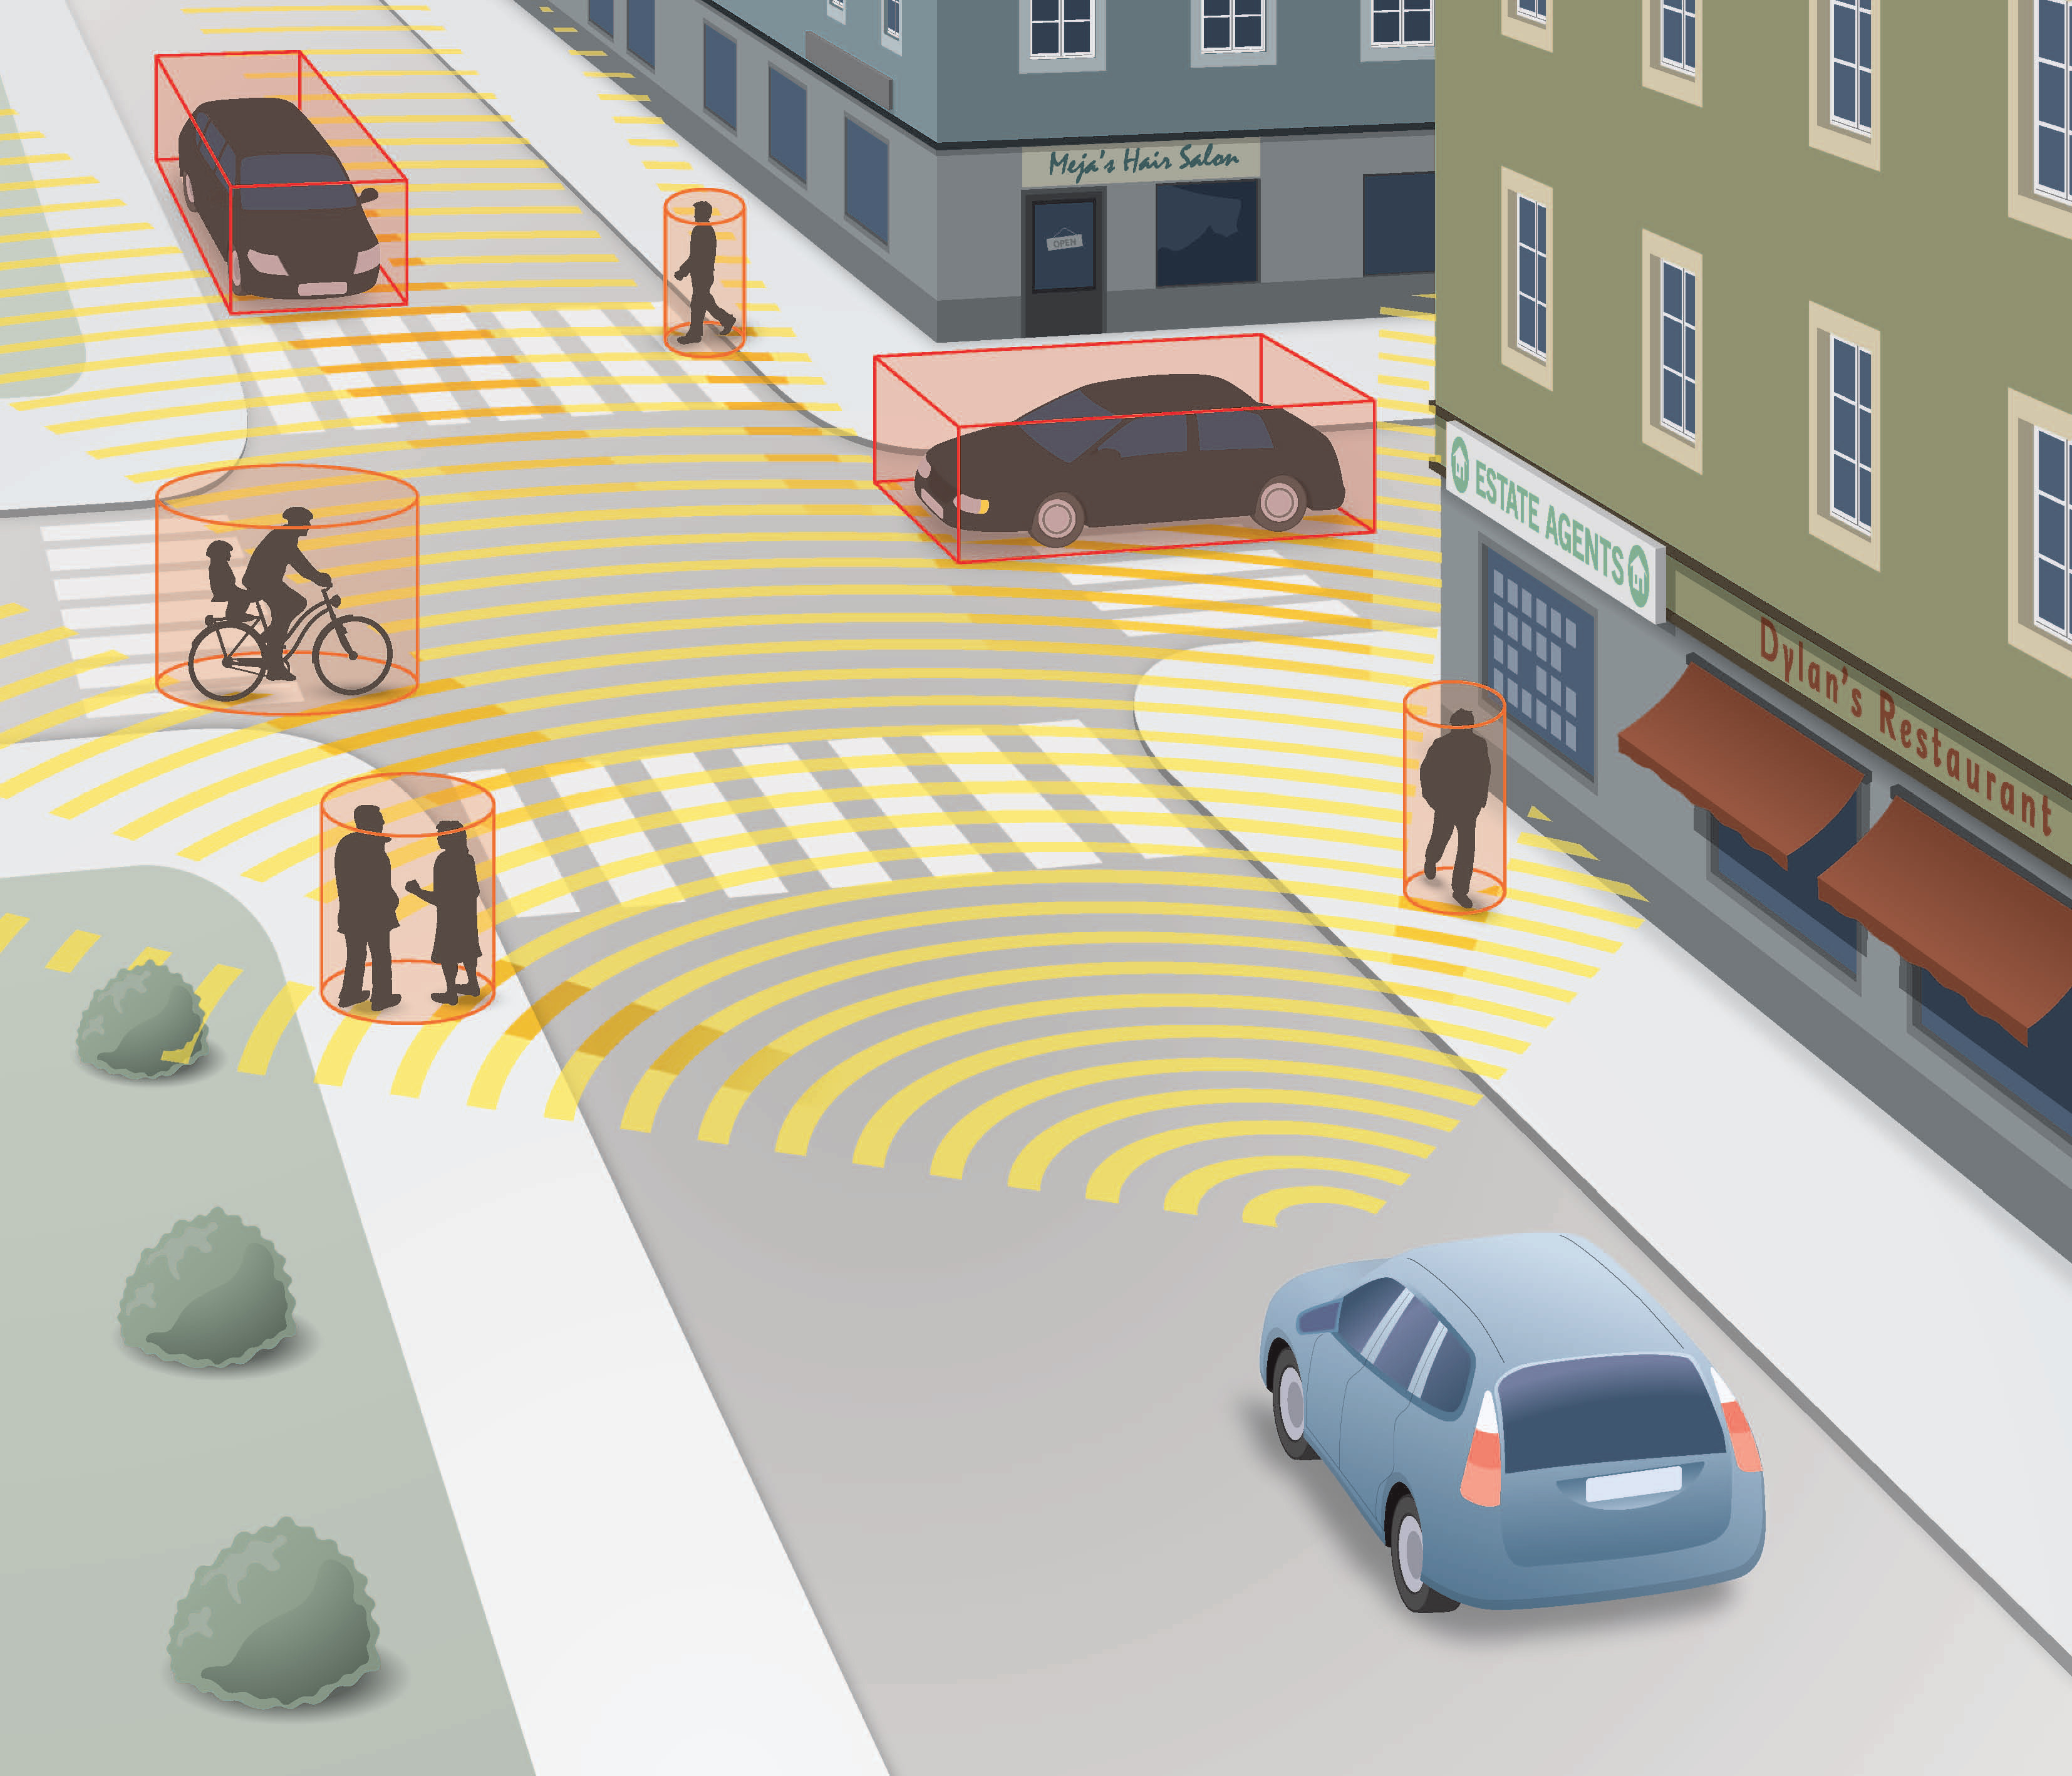
\includegraphics[width=0.7\linewidth]{figure/cover}
% \end{figure}

% Cover text
\mbox{}
\vfill
\renewcommand{\familydefault}{\sfdefault} \normalfont % Set cover page font
\textbf{{\Huge 	Poisson Multi-Bernoulli Filter for	\\[0.2cm] 
				Multiple Extended Target Tracking }} 	\\[0.5cm]
{\Large }\\[0.5cm]
Master's thesis in Communication Engineering \setlength{\parskip}{1cm}

{\Large YUXUAN XIA} \setlength{\parskip}{2.9cm}

Department of Signals and Systems \\
\textsc{Chalmers University of Technology} \\
Gothenburg, Sweden 2017

\renewcommand{\familydefault}{\rmdefault} \normalfont % Reset standard font
\end{titlepage}


% BACK OF COVER PAGE (BLANK PAGE)
\newpage
\restoregeometry
\thispagestyle{empty}
\mbox{}


% TITLE PAGE
\newpage
\thispagestyle{empty}
\begin{center}
	\textsc{\large Master's thesis 2017:NN}\\[4cm]		% Report number given by department 
	\textbf{\Large Poisson Multi-Bernoulli Filter for Multiple Extended Target Tracking} \\[1cm]
% 	{\large A Subtitle that can be Very Much Longer if Necessary}\\[1cm]
	{\large YUXUAN XIA}
	
	\vfill	
	% Logotype on titlepage	
	\begin{figure}[H]
	\centering
	% Remove the following line to remove the titlepage logotype
	
\includegraphics[width=0.2\pdfpagewidth]{figure/auxiliary/logo_eng.pdf} \\	
	\end{figure}	\vspace{5mm}	
	
	Department of Signals and Systems \\
	\emph{Division of Communication Systems}\\
% 	Name of research group (if applicable)\\
	\textsc{Chalmers University of Technology} \\
	Gothenburg, Sweden 2017 \\
\end{center}


% IMPRINT PAGE (BACK OF TITLE PAGE)
\newpage
\thispagestyle{plain}
\vspace*{4.5cm}
Poisson Multi-Bernoulli Filter for Multiple Extended Target Tracking\\
% A Subtitle that can be Very Much Longer if Necessary\\
YUXUAN XIA \setlength{\parskip}{1cm}

\copyright ~ YUXUAN XIA, 2017. \setlength{\parskip}{1cm}

Supervisor: Karl Granst{\"o}m, Lennart Svensson, Department of Signals and Systems\\
Examiner: Lennart Svensson, Department of Signals and Systems \setlength{\parskip}{1cm}

Master's Thesis 2017:NN\\	% Report number given by department 
Poisson Multi-Bernoulli Filter for Multiple Extended Target Tracking\\
% Name of research group (if applicable)\\
Chalmers University of Technology\\
SE-412 96 Gothenburg\\
Telephone +46 31 772 1000 \setlength{\parskip}{0.5cm}

\vfill
% Caption for cover page figure if used, possibly with reference to further information in the report
Cover: Urban scene with multiple moving objects. The blue vehicle must be able to keep track of all the moving objects, e.g., pedestrians, cars, bicycles, in order to operate safely. Figure source from \cite{rfsextended}. \setlength{\parskip}{0.5cm}

Typeset in \LaTeX \\
Printed by [Chalmers University of Technology]\\
Gothenburg, Sweden 2017



% ABSTRACT
\newpage
% CREATED BY DAVID FRISK, 2016
Poisson Multi-Bernoulli Filter for Multiple Extended Target Tracking\\
% A Subtitle that can be Very Much Longer if Necessary\\
YUXUAN XIA\\
Department of Signals and Systems\\
Chalmers University of Technology
\setlength{\parskip}{0.5cm}

\thispagestyle{plain}			% Supress header 
\setlength{\parskip}{0pt plus 1.0pt}
\section*{Abstract}
Multiple target tracking is a core task in the field of autonomous driving. Due to the rapid development of high-resolution sensors, e.g., near-field radar and lidar, a target may occupy multiple sensor cells on any given scan. Solving the multiple extended target tracking problem is mainly complicated by the unknown correspondence between targets and measurements that a huge number of data association events need to be considered.

~\\
In this thesis work, a Poisson multi-Bernoulli (PMB) filter for multiple extended target tracking is proposed, within which the extended targets are modelled using gamma Gaussian inverse Wishart  distributions. The PMB filter is based on the Poisson multi-Bernoulli mixture (PMBM) conjugate prior and approximates the posterior PMBM as a single PMB via variational approximation. The data association problem is handled by iteratively sampling from the posterior distribution that directly maximizes the desired likelihood function. 

~\\
The PMB filter is compared to the PMBM filter and Probability Hypothesis Density filter in simulated scenarios with performance assessed using the generalized optimal sub-pattern assignment (GOSPA) metric. Simulation results show that the PMB filter arguably provides the best overall performance regarding GOSPA error and computational time. 



% KEYWORDS (MAXIMUM 10 WORDS)
\vfill
Keywords: multiple target tracking, extended targets, random finite sets, inverse Wishart, Bayesian inference, Monte Carlo methods, sampling methods, variational approximation.

\newpage				% Create empty back of side
\thispagestyle{empty}
\mbox{}

% ACKNOWLEDGEMENTS
\newpage
% CREATED BY DAVID FRISK, 2016
\thispagestyle{plain}			% Supress header
\section*{Acknowledgements}


\vspace{1.5cm}
\hfill
Yuxuan Xia, Gothenburg, August 2017

\newpage				% Create empty back of side
\thispagestyle{empty}
\mbox{}


% TABLE OF CONTENTS
\newpage
\tableofcontents

% OTHER FRONTMATTER
% List of figures (add to table of contents)
\cleardoublepage
\addcontentsline{toc}{chapter}{\listfigurename} 
\listoffigures
% List of tables (add to table of contents)
\cleardoublepage
\addcontentsline{toc}{chapter}{\listtablename}  
\listoftables


% START OF MAIN DOCUMENT
\cleardoublepage
\setcounter{page}{1}
\pagenumbering{arabic}			% Arabic numbering starting from 1 (one)
\setlength{\parskip}{0pt plus 1pt}

% INTRODUCTION
% CREATED BY DAVID FRISK, 2016
\chapter{Introduction}
The development of autonomous driving has attracted an enormous amount of interest in research during last decades. In order for a self-driving vehicle to be deployed in real-world environments, it must be capable of reliably and efficiently modelling static as well as dynamical obstacles, e.g., landmarks, pedestrians and other nearby moving vehicles. The process of estimating the number of targets and their individual states based on a sequence of noise-corrupted measurements including missed detections and false alarms is denoted as multiple target tracking (MTT). Traditionally, MTT algorithms have been tailored with the ``point target'' assumption that each target is modelled as a point without spatial extent, and that each target gives rise to at most one measurement per time scan. Popular solutions to MTT are the joint probabilistic data association (JPDA) filter \cite{jpda}, multiple hypothesis tracker (MHT) \cite{mht} and approaches based on random finite sets (RFS) \cite{rfs}.

~\\
However, the high-resolution feature of modern radar and lidar sensors equipped on self-driving vehicles makes the ``point target'' assumption unrealistic, since it is common that targets may occupy several sensor resolution cells. The tracking of such a target leads to the so-called extended target tracking problem, and the objective is to recursively determine the time-varying shape and kinematic parameters of the target. In extended target tracking, a non-standard measurement model is needed to model the number and the spatial distribution of generated measurements for each target. A common choice for modelling the number of measurements is the inhomogeneous Poisson Point Process (PPP), proposed in \cite{ppp}. As for the modelling of the spatial distribution, two popular models are the Random Hypersurface Models \cite{hypersurface} and the Gaussian inverse Wishart (GIW) approach \cite{randomMatrix,randomMatrix2}. The former is designed for general star-convex shape; the latter relies on the elliptic shape that it models the spatial distribution of target-generated measurements as Gaussian with unknown mean and covariance. The Gamma GIW (GGIW) model \cite{phdextended,cphdextended} is an extension of the GIW model by incorporating the estimation of target measurement rates. 

~\\
Solving the MTT problem is mainly complicated by the unknown correspondence between targets and measurements, known as data association. Unfortunately, the problem of data association can be even more challenging in multiple extended target tracking, since each target can generate multiple measurements per time scan. In previous work \cite{phdextended,pmbmextended,pmbmextended2}, the data association can be split into two parts: first, clustering methods are used to find multiple partitions of the set of measurements; second, assignment methods are used to assign each measurement cell to a target or a clutter source. In the recently presented work \cite{soextended}, a stochastic optimization (SO) method is proposed that directly maximises the multi-target likelihood function and solves the data association problem in a single step. It has been demonstrated in \cite{soextended} that the SO approach has improved performance in comparison to methods which involve clustering and assignment. 

~\\
Many of the existing multiple extended target tracking algorithms are based on RFS with the distribution of target-generated measurements modelled as GIW or GGIW. Developments using RFS have yielded a variety of tracking methods, such as Probability Hypothesis Density (PHD) filter \cite{phdextended2,phdextended3}, Cardinalised PHD (CPHD) filter \cite{cphdextended}, Generalised Labeled Multi-Bernoulli (GLMB) filter \cite{lmbextended} and its approximation Labeled Multi-Bernoulli (LMB) filter \cite{lmbextended} as well as the Poisson Multi-Bernoulli Mixture (PMBM) filter \cite{pmbmextended,pmbmextended2}. The computational efficient PHD and CPHD filters are based on moment approximations of posterior distributions, while the GLMB and PMBM filters are based on conjugate priors that can provide accurate approximations to the exact posterior distributions. In the context of MTT, conjugacy means that if we begin with a multi-target density of a conjugate prior form, then all subsequent predicted and updated multi-target densities will also be of the conjugate prior form. Comparison results in \cite{pmbmextended,lmbextended} have shown that for extended target tracking filters based on conjugate priors outperform the PHD and CPHD filters. Additionally, it should be noted that only the GLMB and LMB filters produce estimates of targets trajectories. In this thesis, the focus is on the estimates of target states.

~\\
A variational Bayesian approach to approximating the PMBM density with a single Poisson multi-Bernoulli (PMB) density was presented in \cite{variational} for point targets tracking. PMB filter is a computationally efficient approximation of PMBM filter, but it is not yet clear how the variational method of \cite{variational} can be used on extended targets tracking. In this thesis, a PMB filter for multiple extended target tracking is presented, which recursively finds the best-fitting PMB of the PMBM posterior by minimising the Kullback-Leibler divergence (KLD). The performance and computational time of the PMB filter are compared to the PHD filter and the PMBM filter in simulated scenarios. Additionally, two other sampling approaches to extended target tracking, namely Gibbs sampling \cite{gibbs} and merge/split Metropolis Hastings (MH) sampling \cite{mergesplit}, are evaluated by comparing the estimation performance and computational time to the approach based on SO. The multi-target filtering performance is assessed using the generalised optimal sub-pattern assignment (GOSPA) metric \cite{gospa}, in which the estimated location and shape error of extended targets are measured using Gaussian Wasserstein Distance \cite{gwmetric}. Compared with the unnormalised OSPA metric \cite{ospa}, the GOSPA metric allows for further breaking down the cardinality mismatch into errors due to missed and false targets. 

~\\
In this work, three different scenarios have been simulated. The first scenario under consideration is tracking of 27 well-spaced targets. In the second scenario, two targets are spatially well separated at the beginning, then move in parallel in close proximity, before separating again towards the end. In the last scenario, three targets are born spatially close to each other and then separate gradually. Various aspects of different filters with different sampling methods to handle the data association problem are analysed in these three scenarios. Though all filters and sampling methods have pros and cons, the PMB filter with stochastic optimization arguably provides the best overall performance regarding GOSPA and computational time. 

~\\
This thesis is organized as follows. The background is presented in Chapter 2. Chapter 3 discusses approaches to solving the data association problem based on Gibbs sampling and MH sampling. The PMB filter for extended target tracking is derived in Chapter 4. Simulation results are presented in Chapter 5 and conclusions are drawn in Chapter 6. 

% \section{Section levels}
% The following table presents an overview of the section levels that are used in this document. The number of levels that are numbered and included in the table of contents is set in the settings file \texttt{Settings.tex}. The levels are shown in Section \ref{Section_ref}.

% \begin{table}[H]
% \centering
% \begin{tabular}{ll} \hline\hline
% Name & Command\\ \hline
% Chapter & \textbackslash\texttt{chapter\{\emph{Chapter name}\}}\\
% Section & \textbackslash\texttt{section\{\emph{Section name}\}}\\
% Subsection & \textbackslash\texttt{subsection\{\emph{Subsection name}\}}\\
% Subsubsection & \textbackslash\texttt{subsubsection\{\emph{Subsubsection name}\}}\\
% Paragraph & \textbackslash\texttt{paragraph\{\emph{Paragraph name}\}}\\
% Subparagraph & \textbackslash\texttt{paragraph\{\emph{Subparagraph name}\}}\\ \hline\hline
% \end{tabular}
% \end{table}

% \section{Section} \label{Section_ref}
% \subsection{Subsection}
% \subsubsection{Subsubsection}
% \paragraph{Paragraph}
% \subparagraph{Subparagraph}



% THEORY
% CREATED BY DAVID FRISK, 2016
\chapter{Background}

\section{Problem Formulation}
An RFS is an unordered finite set of random variables whose cardinality is also a random variable \cite{rfs}. In RFS-based MTT methods, target states and observations are both represented in the form of finite sets. Let the target set at time step $k$ denoted as $X_k = \{x^1_k,...,x^{|X_k|}_k\}$, where random variable $x^i_k$ denotes the state of $i$th target at time step $k$ and the target set cardinality $|X_k|$ is a time-varying discrete random variable. The set of measurements obtained at time $k$ is denoted as $Z_k = \{z^1_k,...,z^{|Z_k|}_k\}$, where the measurement set cardinality $|Z_k|$ is a discrete random variable. Further, the sequence of all the measurement sets received so far up to time $k$ is denoted as $Z^k$. 

~\\
MTT involves using the measurement sets $Z^k$ to estimate the target set $X_k$, which captures the information about the number of targets and individual target states. Let $f_{k|k^{\prime}} (X_k|Z^{k^{\prime}})$ denote the multi-target distribution at time $k$ given all measurement sets up to and including time $k^{\prime}$, and let $f_k(Z_k|X_k)$ denote the multi-target measurement likelihood. Given these definitions, the multi-target Bayes filter propagates the multi-target distribution in time using the Bayes update \cite[p .484]{rfs}
\begin{equation}
    f_{k|k}(X_k|Z^k) = \frac{f_{k}(Z_k|X_k)f_{k|k-1}(X_k|Z^{k-1})} {\int f_{k}(Z_k|X_k)f_{k|k-1}(X_k|Z^{k-1}) \delta X_k},
    \label{eq:update}
\end{equation}
and the Chapman-Kolmogorov prediction \cite[p .484]{rfs}
\begin{equation}
    f_{k+1|k}(X_{k+1}|Z^k) = \int f_{k+1|k}(X_{k+1}|X_k)f_{k|k}(X_k|Z^k)\delta X_k,
    \label{eq:predict}
\end{equation}
where the set integral is defined as \cite[p .361]{rfs}:
\begin{equation}
    \int f(X)\delta X \triangleq f(\emptyset) + \sum_{n=1}^{\infty}\frac{1}{n!}\int f(\{x_1,...,x_n\})d(x_1,\dotsb,x_n).
    \label{eq:setintegral}
\end{equation}



\section{Modeling}
In this section, some forms of RFS distributions are introduced first. The standard target transition model and the extended target model are then presented. 

\subsection{Random finite set modeling}
\subsubsection{Poisson point process}
A non-homogeneous PPP
with intensity function $D(x)=\mu f(x)$ has RFS density function \cite{pmbmextended2}
\begin{equation}
    f(X) = e^{-\int D(x)dx}\prod_{x\in X}D(x)=e^{-u}\prod_{x\in X}\mu f(x),
    \label{eq:poisson}
\end{equation}
where $\mu$ is the Poisson rate and $f(x)$ is the spatial distribution. The set cardinality $|X|$ is Poisson distributed, and all the variables $x\in X$ are independent and identical distributed (IID). PPPs are often used to model clutter measurements and extended target measurements.

\subsubsection{Bernoulli process}
A Bernoulli process with existence probability $r$ and probability density function (pdf) $f(x)$ has RFS density
\begin{equation}
f(X) = 
\begin{cases}
    1-r,& X=\emptyset\\
    r\cdot f(x),& X=\{x\}\\
    0,& |X| > 1
\end{cases}
\label{eq:bernoulli}\\
\end{equation}
The cardinality $|X|$ is Bernoulli distributed with parameter $r$. This can be interpreted to mean that set $X$ has a probability $1-r$ of being empty, and a probability $r$ of containing a single variable with pdf $f(x)$. In MTT, a Bernoulli process can be used to capture the uncertainty of a single target regarding both its existence $r$ and its state $x$. 

\subsubsection{Multi-Bernoulli process}
An MB process $X$ is a discrete union of independent Bernoulli processes $X^i$, i.e., $X = \uplus_{i\in\mathbb{I}}X^i$, where $\mathbb{I}$ is the index set of Bernoulli components. The RFS density of an MB process can be represented as \cite{pmbmextended2}
\begin{equation}
f(X) = 
\begin{cases}
\sum_{\uplus_{i\in\mathbb{I}}X^i=X}\prod_{i\in\mathbb{I}}f^i(X^i), & |X| \leq |\mathbb{I}| \\
0, & |X| > |\mathbb{I}|
\end{cases}
\label{eq:mb}
\end{equation}
In MTT, targets are typically assumed to be independent. Thus, multiple targets can be naturally represented through an MB process. 


\subsection{Dynamics model}
In this thesis, it is assumed that targets arrive according to a PPP, independently of existing targets. At each time step, targets remain with a probability of survival $p^S_k(x)$. Targets depart according to IID Markov processes with probability $1-p^S_k(x)$. Targets evolve independently from time step $k$ to time step $k+1$ according to IID Markov processes with transition density $f_{k+1|k}(x_{k+1}|x_{k})$. 

\subsection{Extended target measurement model}
The set of measurements $Z_k$ is the union of a set of clutter measurements and sets of target-generated measurements. The clutter is modelled as a PPP with Poisson rate $\lambda$ and spatial distribution $c(z)$, independent of targets and any target-generated measurements. Each extended target may give rise to multiple measurements with the state dependent probability of detection $p^D(x_k)$. If the extended target is detected, the target-generated measurements are modelled as a PPP with Poisson rate $\gamma(x_k)$ and the spatial distribution $\phi(z|x_k)$, independent of all other targets and their corresponding generated measurements. 

~\\
The extended target set measurement likelihood for a non-empty set of measurements is the product of target detection probability and the PPP density of target-generated measurements \cite{pmbmextended2}
\begin{equation}
    f(Z_k|x_k) = p^D(x_k)e^{-\gamma(x_k)}\prod_{z_k\in Z_k}\gamma(x_k)\phi(z_k|x_k).
\end{equation}
For an extended target state $x_k$, the effective detection probability is the product of the target detection probability and the probability that the target generates at least one measurement, which is $1-e^{-\gamma(x_k)}$. Then the effective probability of missed detection can be calculated accordingly as
\begin{equation}
    q^D(x_k) = 1 - p^D(x_k) + p^D(x_k)e^{-\gamma(x_k)},
\end{equation}
which is also the measurement likelihood for an empty measurement set.

\subsection{GGIW model}
In the GGIW model, the extended target state $x_k$ is modelled as 
\begin{equation}
    x_k=(\gamma_k,\xi_k,\chi_k),
\end{equation}
where positive random variable $\gamma_k$ is the Poisson rate that models the average number of measurements generated by the target, the random vector $\xi_k$ describes the kinematic state of the target centroid (e.g., position, velocity, acceleration and turn-rate), and the random covariance matrix $\chi_k$ describes the size and shape of the target. It is assumed that the measurements are Gaussian distributed around the centroid of the target. Since that the gamma distribution is the conjugate prior for the unknown Poisson rate, and that the Gaussian-inverse Wishart distributions are the conjugate priors for Gaussian distributed detections with unknown mean and covariance, the density of the extended target state can be expressed as
\begin{align}
f_{k|k}(x_k) &= \mathcal{GAM}(\gamma_k;\alpha_{k|k},\beta_{k|k})\mathcal{N}(\xi_k;\mathbf{m}_{k|k},P_{k|k})\mathcal{IW}_d(\chi_k;v_{k|k},V_{k|k}) \\
&\triangleq \mathcal{GGIW}(\xi_k;\zeta_{k|k}),
\end{align}
where $\zeta_{k|k} = \{\alpha_{k|k},\beta_{k|k},\mathbf{m}_{k|k},P_{k|k},v_{k|k},V_{k|k}\}$ is the set of GGIW density parameters; $\mathcal{GAM}(\gamma;\alpha,\beta)$ is the gamma pdf with shape $\alpha>0$ and inverse scale $\beta>0$; $\mathcal{N}(\xi;\mathbf{m},P)$ is the Gaussian pdf with mean $m$ and covariance $P$; $\mathcal{IW}_d(\chi;v,V)$ is the inverse Wishart pdf with degrees of freedom $v>2d$ and scale matrix $V$ of dimension $d$.




% \section{Extended target state space model}
% Many approaches are available for modelling the spatial distribution of a single extended target, see \cite{extendedoverview} for a comprehensive discussion. In this thesis, random matrix model \cite{randomMatrix,randomMatrix2} is used, which implies the target shape is an ellipse. The random matrix approach models the extended target state as the combination of a Poisson rate scalar $\gamma_k$, a kinematic state vector $\bold{\xi}_k$ and an extent matrix $S_k$.

%\lstset{language=Matlab}
% \begin{lstlisting}[frame=single]
% % Generate x- and y-nodes
% x=linspace(0,1); y=linspace(0,1);

% % Calculate z=f(x,y)
% for i=1:length(x)
%  for j=1:length(y)
%   z(i,j)=x(i)+2*y(j);
%  end
% end
% \end{lstlisting}
\section{PMB for Point Target Tracking}
The PMBM MTT conjugate prior was developed for point target in \cite{pmbmpoint,pmbmpoint2}. A variational Bayesian approach to approximating the MB mixture (MBM) density with a single MB density was presented in \cite{variational}, leading to the so-called PMB filter. In this section, a background on the PMB filter for multiple point target tracking is presented. The reader is referred to \cite{variational,pmbmpoint} for detailed analytic derivations and mathematical expressions.

\subsection{The PMBM conjugate prior}
The PMBM is a linear combination of independent PPP and MBM components with the following form
\begin{equation}
    f(X_k) = \sum_{X_k^u\uplus X_k^d=X_k}f^{u}(X_k^u)f^{d}(X_k^d),
\label{eq:pmbm}
\end{equation}
where $X^u$ and $X^d$ correspond to undetected targets and detected targets respectively. Let $\mathbb{J}$ be the index set of MB components in the MBM, and $\mathbb{I}^j$ be the index set of Bernoulli components in the $j$th MB. For targets $X^d$ that have already been detected, their distributions can be described as an MBM of the form \cite{pmbmextended2}:
\begin{subequations}
\begin{align}
    f^{d}(X^d_k) &= \sum_{j\in\mathbb{J}}\mathcal{W}^jf^j(X^d),\\
    f^j(X^d) &= \begin{cases}
\sum_{\uplus_{i\in\mathbb{I}^j}X^i=X^d}\prod_{i\in\mathbb{I}^j}f^{j,i}(X^i), & |X^d| \leq |\mathbb{I}| \\
0, & |X^d| > |\mathbb{I}|
\end{cases}
\end{align}
\label{eq:mbm}
\end{subequations}
where $f^{j,i}(\cdot)$ is a Bernoulli process, defined in (\ref{eq:bernoulli}), and weight $\mathcal{W}^j$ is the probability of $j$th MB component, satisfying $\sum_{j\in\mathbb{J}}\mathcal{W}^j = 1$.


~\\
Each of the MB components in MBM typically corresponds to a particular global association hypothesis for the detected targets \cite{pmbmpoint}, with its probability indicated by the corresponding weight. Each global association hypothesis is made up of single target hypotheses on each target \cite{pmbmpoint}. One single target hypothesis can incorporate events, including that the target never existed, that the target existed before and that the target continues to exist, represented via Bernoulli process. Missed detection may occur on some proportions of targets that are hypothesised to be born. A target that is hypothesised to exist but has never been detected is treated as an unknown target \cite{pmbmpoint}. The distribution of unknown targets $f^u(X^u)$ is modelled as the PPP component, defined in (\ref{eq:poisson}).

\subsection{Variational MB}
A PMB is a union of a PPP describing unknown targets and an MB process describing already detected targets. In PMB recursion, the PMB density is preserved in prediction step, whereas the MB component becomes an MBM due to data association. A variational approximation method was presented in \cite{variational} to obtain the best-fitting MB $g(X)$ that minimises the Kullback-Leibler (KL) divergence from the MBM distribution $f(X)$:
\begin{equation}
\underset{g}{\arg\min}\int f(X)\log\frac{f(X)}{g(X)} = \underset{g}{\arg\max}\int f(X)\log g(X)dX.
\label{eq:kl}
\end{equation}


~\\
An approximate solution is based on minimizing the upper bound of (\ref{eq:kl}), using the variational Bayesian expectation-maximization (EM) approach. The correspondence between the Bernoulli distribution in the MBM and the Bernoulli distribution in the best-fitting MB distribution is treated as missing data. The upper bound to the objective of (\ref{eq:kl}) is given by \cite{variational}
\begin{equation}
D_{UB}(f(X)||g(X))= -\sum_{j\in\mathbb{J},\pi\in\Pi_N}\mathcal{W}^jq_j(\pi)\sum_{i=1}^N\int f^{j,i}(X^i)\log g^{\pi(i)}(X^i)\delta X^i,
\end{equation}
with the assumption that each MB has the same number of Bernoulli components  $N$, i.e., $|\mathbb{I}^j|=N$ for $j\in\{1,...,|\mathbb{J}|\}$, and that the missing data $q_j(\pi)$ is constrained to vary only with the $j$th MB component. The missing data satisfies $q_j(\pi) \geq 0$ and $\sum_{\pi\in\Pi}q_j(\pi)=1$, where $\Pi$ is the set of all ways to assign the Bernoulli components in $f^j(X)$ to the Bernoulli components in $g(X)$. The EM process proceeds by alternating between estimating $q_j(\pi)$ and optimizing $g(X)$. 


~\\
Further, it is shown in \cite{variational} that this optimization problem can be solved approximately as:
\begin{equation}
    \min\limits_{q(h,j)\in\mathcal{M}}-\sum^N_{j=1}\int \Bigg(\sum_{h\in\mathcal{H}}q(h,j)f_{h}(X)\Bigg)\cdot\log g^j(X)\delta X,
    \label{eq:qhj}
\end{equation}
where $\mathcal{H}$ is the index set of all the unique Bernoulli components in $f(X)$, and $q(h,j)$ is the probability that a Bernoulli component $f_h(X)$ in $f(X)$ is assigned to the $j$th Bernoulli component of $g(X)$. $\mathcal{M}$ is an approximated polytope needed for tractability
\begin{equation}
    \mathcal{M} = \Bigg\{q(h,j)\geq0\Bigg|\sum_{h\in\mathcal{H}}q(h,j)=1 ~\forall~ j\in\{1,...,N\},\sum^N_{j=1}q(h,j)=p_h ~\forall~ h\in\mathcal{H}\Bigg\},
\end{equation}
where $p_h$ can be interpreted as the probability of Bernoulli component $f_h(X)$ in $f(X)$ is assigned to the approximated MB $g(X)$. In this case, the E-step reverts to a Linear programming (LP) \cite{variational}. The variational MB algorithm is initialized with
\begin{equation}
p_j(h) = \sum\limits_{f^j(X)|f^{j,i}(X)=f_h(X)}w_j,
\end{equation}
which can be approximately calculated using loopy belief propagation (LBP) \cite{lbp}.

\section{PMBM for Extended Target Tracking}
The PMBM model was developed for multiple extended target tracking in \cite{pmbmextended,pmbmextended2,soextended}. The data association problem is very challenging in extended target tracking. It is unknown that which measurements are from targets and which are clutter, and that which target generated which measurement. In previous work \cite{pmbmextended,pmbmextended2}, the data association is split into two parts, called partitioning and assignment. The recent work \cite{soextended} has dealt with the data association using a SO approach that it works directly on maximizing the likelihood. In this section, a summary of the results in these papers is presented. The reader is referred to \cite{pmbmextended,pmbmextended2,soextended} for more implementation details.  

% \subsection{Data association event in the PMBM filter}
% The data association events in the PMBM filter for multiple extended target tracking typically include the following three parts \cite{pmbmextended2}:
% \begin{itemize}
%     \item The set of measurements $Z$ are divided into two parts: $Y$ and $Z\backslash Y$. $Y$ corresponds to measurements that are either clutter or generated by possible unknown targets, while $Z\backslash Y$ corresponds to measurements that are generated by previous detected targets.
%     \item The set of measurements $Y$ is further partitioned into subsets called cells. Each measurement cell corresponds to either clutter or an unknown target.
%     \item The set of measurements $Z\backslash Y$ is also partitioned into cells. Each measurement cell contains measurements generated by a previous detected target, but the exact correspondence is unknown. 
% \end{itemize}

\subsection{The GGIW-PMBM filter implementation}
The conjugacy of GGIW-PMBM filter for extended target tracking has been proved in \cite{pmbmextended2}. The filter propagates the GGIW-PMBM density parameters in time recursively via a prediction step and an update step. In the prediction step, the MB describing previously existed tracks and the PPP describing unknown targets are predicted individually. By having a Poisson birth model, the PPP for new born targets can be easily incorporated into the predicted PPP. 

~\\
In the update step, the PPP and the MBM are updated independently. Two single target hypotheses are created for each measurement cell, and then the PPP intensity is updated by the missed detection probability. The first single target hypothesis covers the case that the measurement cell is associated with a previous target so that this hypothesis has zero existence probability and the corresponding pdf of the Bernoulli distribution has no effect. The second single target hypothesis covers the case that the measurement cell corresponds to a new target, or in the case of the measurement cell containing only one measurement, either a new target or clutter.  

~\\
The density for a target detected for the first time is multi-modal, with one mode for each GGIW component in the predicted PPP density. Mixture reduction can be used to reduce this to a uni-modal GGIW density \cite{phdextended,gammareduction}. For targets surviving from previous time steps, new single target hypotheses are included from missed detection, or updates of previous hypotheses using one of the measurement cells. 
In both PPP and MBM updating, Two new GGIW components are updated for a GGIW component that is not detected. The first is resulted from a missed detection with probability $1-p^D(x)$. The second is because the target generates zero detections. Since only the gamma parameters are different in these two GGIW components, gamma mixture reduction \cite{gammareduction} can be used to reduce this to a single mode GGIW density. 

\subsection{Data association in the PMBM filter}
The data association events in the PMBM filter include partitioning the measurements into measurement cells and associating each measurement cell to a previous detected target or an unknown target. Let $\mathbb{M}_k$ denote the index set of measurements at time step $k$, and $\mathcal{A}^j$ denote the space of all the data associations for the $j$th predicted global association hypothesis. Then $\mathbb{M}_k\cup\mathbb{I}^j_{k|k-1}$ is the union of measurement index set and target index set for the $j$th predicted hypothesis. A data association $A\in\mathcal{A}^j$ is a partition of $\mathbb{M}_k\cup\mathbb{I}^j_{k|k-1}$ into non-empty disjoint subsets $C\in A$, called index cells \cite{pmbmextended2}. An index cell $C$ can consist of a target index $i_C$ and measurement indices of a measurement cell $\mathbf{C}_C$. An index cell can also be formed only be measurement indices of a measurement cell, which corresponds to a possible newly detected target. In addition, an index cell can be formed only by a target index, which means that the corresponding target is miss-detected. 

~\\
In the PMBM update step, each possible data association will result in a MB component in the updated MBM. The likelihood of data association $A\in\mathcal{A}^j$ can be expressed as \cite{pmbmextended2}:
\begin{equation}
\mathcal{L}^{j,A}_{k|k-1}=\prod_{\underset{\underset{C\cap \mathbb{M}_k\neq \emptyset}{C\cap \mathbb{I}^j_{k|k-1}=\emptyset}}{C\in A:}}\mathcal{L}^b_{\mathbf{C}_C}\prod_{\underset{\underset{C\cap \mathbb{M}_k\neq \emptyset}{C\cap \mathbb{I}^j_{k|k-1}\neq\emptyset}}{C\in A:}}\frac{\mathcal{L}^{j,i_C}_{\mathbf{C}_C}}{\mathcal{L}^{j,i_C}_{\emptyset}}\prod_{i\in\mathbb{I}^j_{k|k-1}}\mathcal{L}^{j,i}_{\emptyset},
\end{equation}
where $\mathcal{L}^b_{\mathbf{C}_C}$ is the likelihood that measurement cell $\mathbf{C}_C$ is associated to a clutter or an unknown target, $\mathcal{L}^{j,i_C}_{\mathbf{C}_C}$ is the likelihood that $\mathbf{C}_C$ is associated to target $i_C$ and $\mathcal{L}^{j,i}_{\emptyset}$ is the likelihood that the $i$th target is not detected. Detail expressions of these three likelihoods can be found in \cite{pmbmextended2}. Let $\mathcal{W}^j_{k|k-1}$ denote the weight of the $j$th predicted global association hypothesis, then the updated weight with data association $A\in\mathcal{A}^j$ can be written as
\begin{equation}
\mathcal{W}^{j,A}_{k|k}\propto \mathcal{W}^{j}_{k|k-1}\mathcal{L}^{j,A}_{k|k-1},
\end{equation}
where the proportionality denotes that normalization is required to ensure
\begin{equation}
    \sum_{j\in\mathbb{J}}\sum_{A\in\mathcal{A}^j}\mathcal{W}^{j,A}_{k|k}=1.
\end{equation}

\subsection{Approximations of the data association problem}
Due to the large number of data association hypotheses generated in the update step, the number of PMBM parameters increases rapidly as more data is observed. Since it is not tractable to compute all the possible components, efficient reduction methods need to be used to keep the number of MB components remain at a tractable level. 


\subsubsection{Group gating}
Given the prediction in the PMBM form, it is possible to apply the full PMBM update directly. However, it is more efficient to separate the targets and measurements into approximately independent sub-groups by exploiting the spatial distributions of targets. Gating \cite[Sec. 2.2.2.2]{gating} is used to group targets and measurements. Groups are formed based on targets which share at least one measurement. Group gating enables updates to be performed for each group in parallel.



\subsubsection{Partitioning and assignment}
In each gating group, Distant Partitioning method \cite{phdextended,phdextended2} is used to generate multiple partitions. For the gating group with only measurements, each measurement cell corresponds to a clutter source or an unknown target. For gating groups with both targets and measurements, all possible mappings of the measurement cells to unknown targets or previously detected targets are considered. 

~\\
If the weights of data association hypotheses are generated in non-decreasing order, the M-best mappings (i.e. highest weights) can be selected without computing the weights of all possible mappings exhaustively. The M-mappings with the highest weights can be found by solving the ranked assignment problem using Murty’s algorithm \cite{murty}. Implementation details, e.g., how to construct the cost function for the association map, can be found in \cite{pmbmpoint2}. Another efficient solution to the assignment problem is based on Gibbs sampling. The Gibbs sampling method has been applied in \cite{gibbsglmb} for truncating the GLMB filtering density. It is shown in \cite{gibbsglmb} that the Gibbs sampler based solution has a linear complexity in the number of measurements whereas deterministic ranked assignment solutions are cubic at best. 


\subsubsection{Stochastic optimization}
Instead of solving the data association problem in two separate steps, i.e., partitioning and assignment. A SO method is proposed in \cite{soextended}, which solves the problem in a single step and works directly with the likelihood. It has been proved in \cite{soextended}, the SO method outperforms previous work based on partitioning in scenario where two or more targets are spatially close. 

~\\
The algorithm is initialized by defining as assignment vector $\boldsymbol{\varphi}$ of length $|Z_k|$, indicating which sources the measurements are associated to. If entry $\varphi_m\in\mathbb{I}^j_{k|k-1}$, then the $m$th measurement is associated to a detected target with index $\varphi_m$ for the $j$th predicted global association hypothesis. Otherwise, the $m$th measurement is associated to a clutter or an unknown target. The corresponding data association $A(\boldsymbol{\varphi})$ can be obtained by forming subsets of the measurements indices having equal assignments. A target index is also included in $A(\boldsymbol{\varphi})$ if only $\varphi_m\in\mathbb{I}^j_{k|k-1}$. 

~\\
In each iteration of the sampling, a measurement index is randomly selected. The possible actions can be taken include moving the selected measurement to an existing cell or a new cell, merging the selected cell with an existing cell and splitting the selected cell into two new cells. Given an assignment at the $t$th iteration, the probability resulting from an action $a$ is given by the relative likelihood \cite{soextended}:
\begin{equation}
    P\{\boldsymbol{\varphi}^{(t+1)}=\boldsymbol{\varphi}^{(t)}(a)\mid\boldsymbol{\varphi}^{(t)}\} = \frac{\mathcal{L}^{(t)}_a}{\sum_{a^{\prime}}\mathcal{L}^{(t)}_{a^{\prime}}},
    \label{eq:sampling}
\end{equation}
where $\mathcal{L}^{(t)}_a$ represents the product of the likelihoods of the cells that are affected by the action. Data associations with high posterior probabilities will be sampled more often. After enough number of iterations, a subset of data associations with high likelihoods can be taken from the obtained sequence of data associations. 

% METHODS
% CREATED BY DAVID FRISK, 2016
\chapter{Methods}
Lorem ipsum dolor sit amet, consectetur adipisicing elit, sed do eiusmod tempor incididunt ut labore et dolore magna aliqua. Ut enim ad minim veniam, quis nostrud exercitation ullamco laboris nisi ut aliquip ex ea commodo consequat. Duis aute irure dolor in reprehenderit in voluptate velit esse cillum dolore eu fugiat nulla pariatur. Excepteur sint occaecat cupidatat non proident, sunt in culpa qui officia deserunt mollit anim id est laborum.

% RESULTS
% CREATED BY DAVID FRISK, 2016
\chapter{PMB for Extended Target Tracking}
A PMBM conjugate prior is presented in \cite{pmbmextended,pmbmextended2} that both the prediction and update preserve the PMBM form of the density. The sampling based approaches can be used to handle the data association problem effectively. However, the number of components for a PMBM representation still grows exponentially. One potential direction to further reduce computational complexity is to approximate the MBM part in the PMBM posterior as a single MB. One such approach is to use the variational method proposed in \cite{variational} to find the best-fitting MB that minimizes the KL divergence. 

~\\
In the implementation of the PMB filter for point target tracking \cite{variational}, the variational MB algorithm is initialized with the marginal probabilities $p_i(h)$, as can be approximated efficiently using methods such as LBP. The LBP is formulated by message passing in a bipartite model, in which all target association variables are connected to all measurement association variables \cite{lbp}. The construction of such a graphical model is based on the assumption that a target can generate at most one measurement per time. Thus, it is challenging to design a tractable version of the LBP for approximating the marginal probabilities in extended target tracking. In this chapter, the PMB filter for extended target tracking is presented, along with its GGIW implementation.  

\section{Variational MB for Extended Target}
In this section, a review of algorithms for reduction of Gamma mixtures and inverse Wishart mixtures \cite{phdextended,gammareduction} is presented first, then the explicit expressions of (\ref{eq:mstep}) and (\ref{eq:estep}) in the EM process are given. At last, pseudo-code of a devised variational MB algorithm for extended target is presented. \cite{simplex}. 

\subsection{Mixture reduction}
Theorems describing how a sum of an arbitrary number of Gamma components or inverse Wishart component can be merged into just one Gamma or inverse Wishart component are presented in \cite{gammareduction} and \cite{phdextended} respectively. They are both performed via analytically minimization of the KL divergence
\begin{equation}
    \arg\min\limits_q\text{KL}(p||q) = \int p(x)\log\bigg(\frac{p(x)}{q(x)}\bigg)dx,
\end{equation}
which can be further rewritten as a maximization problem
\begin{equation}
    \arg\min\limits_q\text{KL}(p||q) = \max\limits_q\int p(x)\log q(x)dx.
\end{equation}
\subsubsection{Gamma mixture reduction}
Let $p(\cdot)$ be a weighted sum of Gamma components,
\begin{equation}
    p(\gamma) = \sum_{i=1}^Nw_i\mathcal{GAM}(\gamma;a_i,b_i).
\end{equation}
Let $q(\cdot)$ be the single Gamma component that has the minimum KL divergence to $p(\cdot)$,
\begin{equation}
    q(\gamma) = \bar{w}\mathcal{GAM}(\gamma;a,b)
\end{equation}
where $\bar{w}=\sum_{i=1}^Nw_i$. Then the parameter $b$ is given by
\begin{equation}
    b = \frac{a}{\frac{1}{\bar{w}}\sum_{i=1}^Nw_i\frac{a_i}{b_i}},
\end{equation}
and the parameter $a$ is the solution to
\begin{equation}
    0 = \log a - \psi_0(a) +\frac{1}{\bar{w}}\sum_{i=1}^Nw_i(\psi_0(a_i)-\log b_i)-\log\bigg(\frac{1}{\bar{w}}\sum_{i=1}^Nw_i\frac{a_i}{b_i}\bigg),
    \label{eq:gammamerge}
\end{equation}
where $\psi_0(\cdot)$ is the digamma function. A value for the parameter $a$ can be found by applying a numerical root finding algorithm to (\ref{eq:gammamerge}), e.g., Halley's method \cite{halley}.


\subsubsection{Inverse Wishart mixture reduction}
Let $p(\cdot)$ be a weighted sum of inverse Wishart components, 
\begin{equation}
    p(\chi) = \sum_{i=1}^Nw_i\mathcal{IW}(\chi;v_i,V_i).
\end{equation}
Let $q(\cdot)$ be the single inverse Wishart component that has the minimum KL divergence to $p(\cdot)$,
\begin{equation}
    q(\chi) = \bar{w}\mathcal{IW}(\chi;v,V).
\end{equation}
Then the parameter $V$ is given by
\begin{equation}
    V = \bar{w}(v-d-1)\bigg(\sum_{i=1}^Nw_i(v_i-d-1)V_i^{-1}\bigg)^{-1},
\end{equation}
and the parameter $v$ is the solution to
\begin{multline}
    0 = \bar{w}d\log(v-d-1)-\bar{w}\sum_{j=1}^d\psi_0\bigg(\frac{v-d-j}{2}\bigg) + \bar{w}d\log\bar{w}\\-\bar{w}\log\bigg|\sum_{i=1}^Nw_i(v_i-d-1)V_i^{-1}\bigg|+\sum_{i=1}^N\sum_{j=1}^dw_i\psi_0\bigg(\frac{v_i-d-j}{2}\bigg)-\sum_{i=1}^Nw_i\log|V_i|,
    \label{eq:wishartmerge}
\end{multline}
where $d$ is the dimension of matrix $V$. A value for the parameter $v$ can be found by applying a root finding algorithm to (\ref{eq:wishartmerge}). 



\subsection{EM process for GGIW density}
Assuming the density distributions of Bernoulli components are constrained to be GGIW, (\ref{eq:mstep}) can be replaced by expressions matching the probability of existence and the set of GGIW density parameters $\zeta = \{a,b,\mathbf{m},P,v,V\}$ to the expression in (\ref{eq:mstep}). Since the Gamma, Gaussian and inverse Wishart distributions are mutually independent, the Bernoulli-GGIW form permits closed-form evaluation of (\ref{eq:estep}). Specifically, if
\begin{equation}
    f^{j,i}(X) = \begin{cases}
        1 - r^{j,i}, & X = \emptyset\\
        r^{j,i}\mathcal{GGIW}(\xi^{j,i};\zeta^{j,i}), & X = \{x\}
    \end{cases}
\end{equation}
\begin{equation}
    g^{l}(X) = \begin{cases}
        1 - \hat{r}^{l}, & X = \emptyset\\
        \hat{r}^{l}\mathcal{GGIW}(\hat{\xi}^{l};\hat{\zeta}^{l}), & X = \{x\}
    \end{cases}
\end{equation}
then the M-step reduces to setting:
\begin{subequations}
\begin{align}
    \hat{r}^{l} & = \sum_{j\in\mathbb{J},\pi\in\Pi_N}\mathcal{W}^jq_j(\pi)r^{j,\pi^{-1}(l)},\\
    \hat{\mathbf{m}}^{l} & = \frac{1}{\hat{r}^{l}}\sum_{j\in\mathbb{J},\pi\in\Pi_N}\mathcal{W}^jq_j(\pi)r^{j,\pi^{-1}(l)}\mathbf{m}^{j,\pi^{-1}(l)},\\
    \hat{P}^{l} & = \frac{1}{\hat{r}^{l}}\sum_{j\in\mathbb{J},\pi\in\Pi_N}\mathcal{W}^jq_j(\pi)r^{j,\pi^{-1}(l)}\big\{P^{j,\pi^{-1}(l)}+(\mathbf{m}^{j,\pi^{-1}(l)}-\hat{\mathbf{m}}^{l})(\mathbf{m}^{j,\pi^{-1}(l)}-\hat{\mathbf{m}}^{l})^T\big\},\\
    \hat{a}^l & : \text{solution to (\ref{eq:gammamerge}) with  } w_j=\mathcal{W}^jq_j(\pi)r^{j,\pi^{-1}(l)},\\
    \hat{b}^l & = \frac{\hat{a}^l}{\frac{1}{\hat{r}^{l}}\sum_{j\in\mathbb{J},\pi\in\Pi_N}\mathcal{W}^jq_j(\pi)r^{j,\pi^{-1}(l)}\frac{a^{j,\pi^{-1}(l)}}{b^{j,\pi^{-1}(l)}}},\\
    \hat{v}^l & : \text{solution to (\ref{eq:wishartmerge}) with  } w_j=\mathcal{W}^jq_j(\pi)r^{j,\pi^{-1}(l)},\\
    \hat{V}^l & = \hat{r}^{l}(\hat{v}^{l}-d-1)\bigg(\sum_{j\in\mathbb{J},\pi\in\Pi_N}\mathcal{W}^jq_j(\pi)r^{j,\pi^{-1}(l)}(v^{j,\pi^{-1}(l)}-d-1){V^{j,\pi^{-1}(l)}}^{-1}\bigg)^{-1},
\end{align}
\end{subequations}
while the integral required in the E-step becomes:
\begin{multline}
    -\int f^{j,i}(X)\log g^{l}(X)\delta X = -(1-r^{j,i})\log(1-\hat{r}^l) - r^{j,i}\log\hat{r}^l \\- r^{j,i}\bigg(\int\mathcal{N}(\xi^{j,i};\mathbf{m}^{j,i},P^{j,i})\log\mathcal{N}(\hat{\xi}^l;\hat{\mathbf{m}}^l,\hat{P}^l) + \int\mathcal{GAM}(\gamma^{j,i};a^{j,i},b^{j,i})\\\times\log\mathcal{GAM}(\hat{\gamma}^l;\hat{a}^l,\hat{b}^l) + \int\mathcal{IW}(\chi^{j,i};v^{j,i},V^{j,i})\log\mathcal{IW}(\hat{\chi}^l;\hat{v}^l,\hat{V}^l) \bigg),
    \label{eq:esteplp}
\end{multline}
where
\begin{subequations}
\begin{multline}
    \int\mathcal{N}(\xi^{j,i};\mathbf{m}^{j,i},P^{j,i})\log\mathcal{N}(\hat{\xi}^l;\hat{\mathbf{m}}^l,\hat{P}^l) = -\frac{d}{2}\log(2\pi)-\frac{1}{2}\log|\hat{P}^l|\\-\frac{1}{2}\text{trace}\bigg(\big(P^{j,i}+(m^{j,i}-\hat{m}^l)(m^{j,i}-\hat{m}^l)^T\big)\big(\hat{P}^l\big)^{-1}\bigg),
    \end{multline}
    \begin{multline}
        \int\mathcal{GAM}(\gamma^{j,i};a^{j,i},b^{j,i})\log\mathcal{GAM}(\hat{\gamma}^l;\hat{a}^l,\hat{b}^l) = \hat{a}^l\log\hat{b}^l - \log\Gamma(\hat{a}^l) \\+ (\hat{a}^l-1)(\psi_0(a^{j,i})-\log b^{j,i}) - \hat{b}^l\frac{a^{j,i}}{b^{j,i}},
    \end{multline}
    \begin{multline}
        \int\mathcal{IW}(\chi^{j,i};v^{j,i},V^{j,i})\log\mathcal{IW}(\hat{\chi}^l;\hat{v}^l,\hat{V}^l) = -\frac{(\hat{v}^l-d-1)d}{2}\log2 \\+ \frac{\hat{v}^l-d-1}{2}\log|\hat{V}^l| - \log\Gamma_d\bigg(\frac{\hat{v}^l-d-1}{2}\bigg) - \frac{\hat{v}^l}{2}\bigg(\log|V^{j,i}|-d\log2\\-\sum_{j=1}^d\psi_0\bigg(\frac{v^{j,i}-d-j}{2}\bigg)\bigg) -\frac{1}{2}\text{trace}\big((v^{j,i}-d-1)(V^{j,i})^{-1}\hat{V}^l\big).
    \end{multline}
\end{subequations}

\subsection{Approximation of feasible set}
Whereas the optimization problem in (\ref{eq:vaorigin}) involves missing data $q_j(\pi)$ for every data association, a vastly simplified representation $q(h,l)$ is given in (\ref{eq:qhj}) which specifies the weight of single target hypothesis $h\in\mathcal{H}$ in the new Bernoulli component $g^l(X)$. For an extended target that has already been detected, the single target hypotheses include events that the target is updated by a measurement cell, and that the target is miss-detected (i.e., the corresponding measurement cell is empty). 

% Due to the unknown number of targets detected for the first time, each MB in $f(X)$ may have different number of Bernoulli components. This suggests a devised polytope: 
% \begin{equation}
%     \mathcal{M}^* = \Bigg\{q(h,l)\geq0\Bigg|\sum_{h\in\mathcal{H}}q(h,l)=p_l ~\forall~ l\in\{1,...,N^*\},\sum^{N^*}_{l=1}q(h,l)=p_h ~\forall~ h\in\mathcal{H}\Bigg\}, 
% \end{equation}
% where $N^*$ is the number of Bernoulli components in $g(X)$, which is also the largest number of Bernoulli components that a MB has in $f(X)$. In comparison to (\ref{eq:polytope}), this new polytope also considers the Bernoulli components that correspond to the updates of unknown targets. Given MB components with high likelihoods obtained by solving the data association problem and their corresponding normalized weights, the marginal probabilities $p_l(h)$ can be approximately calculated using (\ref{eq:marginalprob}). 

\subsection{Pseudo-code for GGIW-VMB}
\begin{algorithm}[h!]
  \SetAlgoLined
  \SetKwInOut{Input}{input}\SetKwInOut{Output}{output}
  \Input{$\mathcal{H}, [p_l(h)], [r_h], [a_h], [b_h], [\mathbf{m}_h], [P_h], [v_h], [V_h]$}
  \Output{$q(h,l), [\hat{r}^l], [\hat{a}_l], [\hat{b}_l], [\hat{\mathbf{m}}_l], [\hat{P}_l], [\hat{v}_l], [\hat{V}_l]$}
  $q(h,l)\leftarrow p_l(h) ~\forall~ h\in\mathcal{H}, l\in\{1,...,N^*\}$\;
  $p_h \leftarrow \sum_{l=1}^{N^*}q(h,l)~\forall~ h\in\mathcal{H}$\;
  $p_l\leftarrow \sum_{h\in\mathcal{H}}q(h,l)~\forall~ l\in\{1,...,N^*\}$\;
  \Repeat{\rm{Sufficiently small progress is made in objective of LP from one iteration to next}}{
    $\hat{r}^l \leftarrow \sum_{h\in\mathcal{H}}q(h,l)r_h~\forall~l$\;
    $\hat{\mathbf{m}}^l\leftarrow\frac{1}{\hat{r}^l}\sum_{h\in\mathcal{H}}q(h,l)r_h\mathbf{m}_h~\forall~l$\;
    $\hat{P}^l\leftarrow\frac{1}{\hat{r}^l}\sum_{h\in\mathcal{H}}q(h,l)r_h(P_h+(\mathbf{m}_h - \hat{\mathbf{m}}^l)(\mathbf{m}_h - \hat{\mathbf{m}}^l)^T)~\forall~l$\;
    $\hat{a}^l\leftarrow\text{solution to (\ref{eq:gammamerge}) with }w_h = q(h,l)r_h~\forall~h, l$\;
    $\hat{b}^l\leftarrow\hat{a}^l\hat{r}^l/(\sum_{h\in\mathcal{H}}q(h,l)r_h\frac{a_h}{b_h})~\forall~l$\;
    $\hat{v}^l\leftarrow\text{solution to (\ref{eq:wishartmerge}) with }w_h = q(h,l)r_h~\forall~h, l$\;
    $\hat{V}^l\leftarrow\hat{r}^l(\hat{v}^l-d-1)(\sum_{h\in\mathcal{H}}q(h,l)r_h(v_h-d-1)V_h^{-1})^{-1}$\;
    Calculate $C(h,l)$ using (\ref{eq:esteplp}) $\forall~h,l$\;
    Solve the LP:
    \begin{equation}
        \arg\min\limits_{q(h,l)}\sum_{h\in\mathcal{H}}\sum_{l=1}^{N^*}q(h,l)
        \label{eq:lp}
    \end{equation}
    \begin{subequations}
    \begin{align*}
        \text{subject to}&\sum_{h\in\mathcal{H}}q(h,l)=p_l~\forall~l\\
        &\sum_{l=1}^{N^*}q(h,l) = p_h~\forall~h\\
        &q(h,l)\geq0~\forall~h, l
    \end{align*}
    \end{subequations}
    }
  \caption{GGIW-VMB}
\end{algorithm}
The form of (\ref{eq:lp}) is a network flow LP, referred to as a transportation problem. In this work, the simplex algorithm \cite{simplex} is utilized to solve this problem.

\section{PMB Complexity Reduction}
In the previous section, variational approximation is used to approximate the MBM component of the posterior by a single MB. In this section, the recycling method \cite{recycle} and pruning-based approximations are presented to further decrease the computational cost of the PMB filter. 

\subsection{Recycling}
In the approximated MB, the recycling method of \cite{recycle} can be applied to Bernoulli components with low existence probability. The recycled components are approximated as being Poisson and are incorporated into the PPP representing unknown targets for generating possible new targets in subsequent steps. Thus, the number of Bernoulli components is reduced while the significant information of already detected targets is maintained. In addition, recycling can help recover performance loss due to the pruning of Bernoulli components with small existence probability \cite{lbp}. The benefits of recycling in the PMBM filter and the PMB filter for point target tracking have been demonstrated in \cite{performanceevaluation}.

~\\
Suppose that a Bernoulli component $f(X)$ in the form of (\ref{eq:bernoulli}), with probability of existence $r$ and spatial distribution $f(x)$ is approximated as a PPP
\begin{equation}
    f(X) \approx \tilde{f}(X) = e^{-u}\prod_{x\in X}D(x),
\end{equation}
where $\mu = \int D(x)dx$ is the Poisson rate, and $D(x)$ is the intensity function. The distortion caused by this approximation can be measured by the KL divergence \cite[p. 513]{rfs}
\begin{equation}
    D(f(X)||\tilde{f}(X)) = \int f(X)\log\frac{f(X)}{\tilde{f}(X)}
\end{equation}
As shown in \cite[p. 579]{rfs}, it is optimal to set
\begin{subequations}
\begin{align}
    D(x) &= \mu f(x),\\
    \mu &= r.
\end{align}
\end{subequations}
It was shown in \cite{recycle} that the value of the KL divergence at this optimal choice
\begin{equation}
    D(f(X)||\tilde{f}(X)) = r + (1-r)\log(1-r),
\end{equation}
is very small for existence probability $r$ less than 0.1. Denote $\mathbb{R}$ as the set of indices of Bernoulli components to be recycled. After recycling, the total PPP intensity of unknown targets can be expressed as
\begin{equation}
    D_{k|k}(x) = D^u_{k|k}(x) + \sum_{i\in\mathbb{R}}r^i_{k|k}f^i_{k|k}(x).
\end{equation}

\subsection{Pruning}
For each gating group, solving the data association problem creates multiple updated MB components; these are pruned to only contain the MB components that correspond to $99.99\%$ of the likelihood \cite{pmbmextended2}. An updated MBM is obtained by considering all possible ways to combined the alternative updated MB components for the gating groups. The updated MBM is pruned by discarding MB components with weight smaller than a threshold before implementing variational approximation. For the approximated MB , the Bernoulli components with existence probability smaller than 0.1 are recycled. In the mixture representation of the PPP intensity of unknown targets, the components with weights smaller than a threshold are pruned.  



\section{The GGIW-PMB Filter Implementation}
In this section, the implementation of the GGIW-PMB filter is presented briefly. In the GGIW-PMB filter, the GGIW-PMB density is propagated in time, using a recursion that consists of an update step and a prediction step. The prediction step preserves the GGIW-PMB form, whereas the update step results in a GGIW-PMBM density which is approximated by a GGIW-PMB at each time step. 

~\\
It is assumed that the detection probability $p^D(\cdot)$ and the survival probability $p^S(\cdot)$ are constant, that the clutter Poisson rate $\lambda$ is known, and that the spatial distribution is uniform, $c(z) = A^{-1}$, where $A$ is the area of the surveillance region. The PPP birth intensity is a GGIW mixture with known parameters, given by
\begin{equation}
    D^b_{k+1}(x) = \mu^b_{k+1}\sum^{N^b_{k+1}}_{n=1}w^{b,n}_{k+1}\mathcal{GGIW}(x_{k+1};\zeta^{b,n}_{k+1}),
\end{equation}
and the initial PPP intensity of unknown targets with known parameters is expressed as
\begin{equation}
    D^u_{0}(x) = \mu^u_{0}\sum^{N^u_{0}}_{n=1}w^{u,n}_{0}\mathcal{GGIW}(x_{0};\zeta^{u,n}_{0}).
\end{equation}
The updated density for the PPP of unknown targets has $N^b_{k+1}+N^u_{k+1}$ GGIW components after the prediction. The details of the resulting algorithm are shown in Algorithm \ref{pmbalgorithm}.


\begin{algorithm}[h!]
  \SetAlgoLined
  Initialize PPP intensity of unknown targets: $D^u_0(x) = D^b(x)$\;
  Initialize empty MB: $\mathbb{I}_0 = \emptyset$\;
  \For{$k = 1:\#\rm{total~time~step}$}{
  \textbf{Prediction:}\
  \begin{itemize}
      \item Predict existing PPP intensity, see \cite[Table V]{pmbmextended2}
      \item Incorporate birth intenisty into PPP
      \item Predict MB, see \cite[Table V]{pmbmextended2}
  \end{itemize}
  \textbf{Update:}\\
  Group gating:\\
  For measurements do not fall into any of the gate:
  \begin{itemize}
      \item Clustering (e.g., distant partitioning, sampling based approach)
      \item Do PPP update for each cluster, see \cite[Table VIII]{pmbmextended2}
  \end{itemize}
  \For{\rm{each gating group}}{
    Solving the data association problem\;
    \For{\rm{each MB}}{
        Update Bernoulli components that correspond to detected targets and missed detections, see \cite[Table VII, IX]{pmbmextended2}\;
        Create new Bernoulli components for targets detected for the first time, see \cite[Table VIII]{pmbmextended2}\;
    }
  }
  Combine the updated MB components for all the gating groups\;
  Prune low weight MB components\;
  Merge the MBM into a single MB via variational approximation\;
  Combine the approximated MB with the MB resulted from PPP update of measurements outside the gate\;
  Recycle Bernoulli components with low existence probability\;
  Reduce the GGIW mixture of the Poisson intensity if necessary by pruning\;
  }
  \caption{GGIW-PMB filter}
  \label{pmbalgorithm}
\end{algorithm}

~\\
The density for a target detected for the first time is multi-modal, with one mode for each GGIW component in the predicted PPP density. Mixture reduction can be used to reduce this to a uni-modal GGIW density \cite{phdextended,gammareduction}. For targets surviving from previous time steps, new single target hypotheses are included from missed detection, or updates of previous hypotheses using one of the measurement cells. There are two new GGIW components which are updated for a GGIW component that is not detected in both the PPP and the MBM update. The first is resulted from a missed detection with probability $1-p^D(x)$. The second is because the target generates zero detections. Since only the gamma parameters are different in these two GGIW components, gamma mixture reduction \cite{gammareduction} can be used to reduce this to a single mode GGIW density. Due to the similarity with the implementation of the GGIW-PMBM filter, expressions regarding the prediction and update of undetected PPP, Bernoulli components and MB using GGIW modeling are omitted for brevity, details can be found in \cite{pmbmextended2}. 



% CONCLUSION
% CREATED BY DAVID FRISK, 2016
\chapter{Conclusion}
Lorem ipsum dolor sit amet, consectetur adipisicing elit, sed do eiusmod tempor incididunt ut labore et dolore magna aliqua. Ut enim ad minim veniam, quis nostrud exercitation ullamco laboris nisi ut aliquip ex ea commodo consequat. Duis aute irure dolor in reprehenderit in voluptate velit esse cillum dolore eu fugiat nulla pariatur. Excepteur sint occaecat cupidatat non proident, sunt in culpa qui officia deserunt mollit anim id est laborum.


% REFERENCES / BIBLIOGRAPHY
\cleardoublepage
\addcontentsline{toc}{chapter}{Bibliography}
% CREATED BY DAVID FRISK, 2016
\begin{thebibliography}{69}

\bibitem{Reference} Frisk, D. (2016) A Chalmers University of Technology Master's thesis template for \LaTeX . Unpublished.

\end{thebibliography}



% APPENDICES
\cleardoublepage
\appendix
\setcounter{page}{1}
\pagenumbering{Roman}			% Capitalized roman numbering starting from I (one)

% CREATED BY DAVID FRISK, 2016
\chapter{Appendix 1}
Lorem ipsum dolor sit amet, consectetur adipisicing elit, sed do eiusmod tempor incididunt ut labore et dolore magna aliqua. Ut enim ad minim veniam, quis nostrud exercitation ullamco laboris nisi ut aliquip ex ea commodo consequat. Duis aute irure dolor in reprehenderit in voluptate velit esse cillum dolore eu fugiat nulla pariatur. Excepteur sint occaecat cupidatat non proident, sunt in culpa qui officia deserunt mollit anim id est laborum.




\end{document}